\documentclass[preprint,12pt]{article}
\usepackage[table]{xcolor}
\usepackage{amssymb}
\usepackage{amsmath}
\usepackage{tikz}
\usetikzlibrary{arrows.meta}
\usetikzlibrary{tikzmark, positioning, fit, shapes.misc, shadows}
\usetikzlibrary{arrows}
\usetikzlibrary{decorations.pathreplacing, calc,shapes.geometric}
\tikzset{brace/.style={decorate, decoration={brace}},
  brace mirrored/.style={decorate, decoration={brace,mirror}},
}
\usepackage{xcolor}

\begin{document}

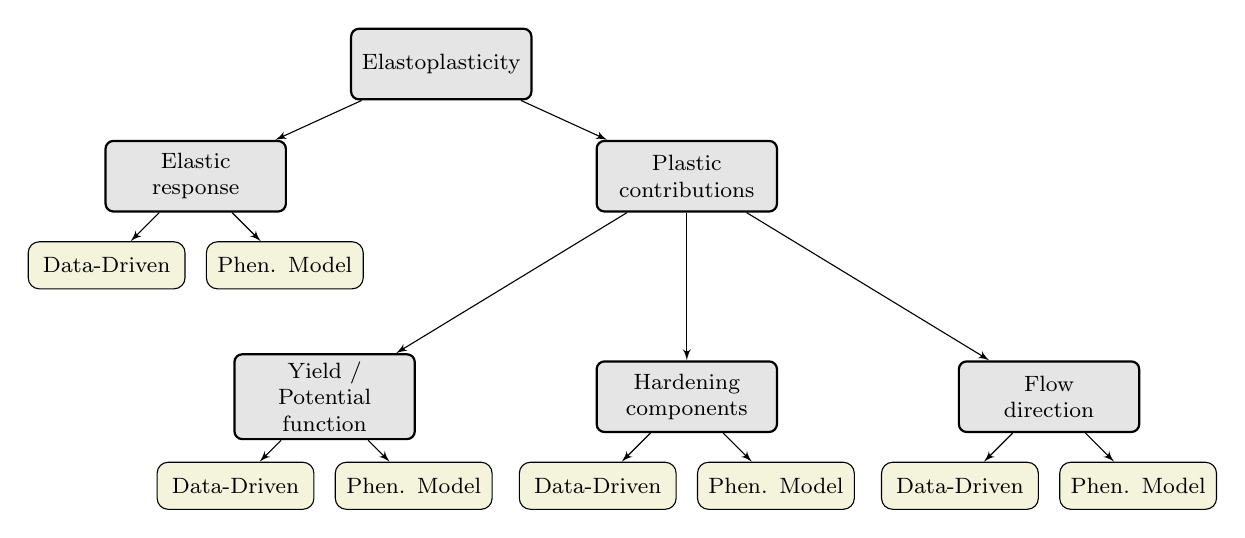
\begin{tikzpicture}[scale=1, every node/.style={transform shape},node distance = 2cm, auto]
% Define block styles
\footnotesize
\tikzstyle{decision} = [diamond, draw, fill=blue!20, 
    text width=4.5em, text badly centered, node distance=3cm, inner sep=0pt]
\tikzstyle{block} = [rectangle, draw, thick, fill=gray!20, text width=7em, text centered, rounded corners=1mm, minimum height=3em]
    
\tikzstyle{block2} = [rectangle, draw, fill=olive!10, text width=6em, text centered, rounded corners, minimum height=2em]
    
\tikzstyle{line} = [draw, -latex']

    
    % Place nodes
    \node [block] (init) {Elastoplasticity};

    \node [block,below left = .5cm and .8cm of init] (elastic) {Elastic\\response};
    \node [block2,node distance = 1.6cm, below left of=elastic] (DataEl) {Data-Driven};
    \node [block2,node distance = 1.6cm, below right of=elastic] (ModelEl) {Phen. Model};
    
    \node [block,below right = 0.5cm and .8cm of init] (plastic) {Plastic \\ contributions};

        \node [block,node distance = 2.8cm, below of=plastic] (hardening) {Hardening\\ components};
            
        \node [block2,node distance = 1.6cm, below left of=hardening] (Datahard) {Data-Driven};
        \node [block2,node distance = 1.6cm, below right of=hardening] (Modelhard) {Phen. Model};

\node [block,node distance = 4.6cm, left of=hardening] (initYield) {Yield / Potential \\ function};

        \node [block2,node distance = 1.6cm, below left of=initYield] (DataYield) {Data-Driven};
        \node [block2,node distance = 1.6cm, below right of=initYield] (ModelYield) {Phen. Model};
        
\node [block,node distance = 4.6cm, right of=hardening] (initflow) {Flow\\ direction};

        \node [block2,node distance = 1.6cm, below left of=initflow] (DataFlow2) {Data-Driven};
        \node [block2,node distance = 1.6cm, below right of=initflow] (ModelFlow2) {Phen. Model};





    % Draw edges
    \path [line] (init) -- (elastic);
    \path [line] (init) -- (plastic);
    
    \path [line] (elastic) -- (DataEl);
    \path [line] (elastic) -- (ModelEl);

    
    \path [line] (plastic) -- (initYield);



    \path [line] (initYield) -- (ModelYield);
    \path [line] (initYield) -- (DataYield);



    \path [line] (plastic) -- (hardening);
    
    \path [line] (hardening) -- (Datahard);
    \path [line] (hardening) -- (Modelhard);


    \path [line] (plastic) -- (initflow);
    
    \path [line] (initflow) -- (DataFlow2);
    \path [line] (initflow) -- (ModelFlow2);


\end{tikzpicture}

\end{document}